%\documentclass[aspectratio=169]{beamer} %para apresentações em widescreen
\documentclass[10pt]{beamer} %para apresentação normal
\logo{
\includegraphics[height=1cm]{Imagens/logon.jpg}\vspace{220pt}}
\newcommand{\nologo}{\setbeamertemplate{logo}{}} % command to set the logo to nothing
\usetheme{default}
\usefonttheme{serif}
\usecolortheme{default}
%%%%%%%%%%%%%%%%%%%%PACOTES EXTRAS%%%%%%%%%%%%%%%%%%%
\usepackage[utf8]{inputenc}
\usepackage[T1]{fontenc}
\usepackage[portuguese, english]{babel}
\usepackage[round]{natbib}
\usepackage{hyperref} 
\usepackage{smartdiagram}
\usepackage{graphicx} % Required for including images
\usepackage{graphics}
\graphicspath{{figures/}} % Location of the graphics files
\usepackage{booktabs} % Top and bottom rules for table
\usepackage[font=small,labelfont=bf]{caption} % Required for specifying captions to tables and figures
\usepackage{amsfonts, amsmath, amsthm, amssymb} % For math fonts, symbols and environments
\usepackage{wrapfig} % Allows wrapping text around tables and figures
\usepackage{ucs}
\usepackage{amsmath}
\usepackage{amsfonts}
\usepackage{amssymb}
\usepackage{amsthm}
\usepackage{times}
\usepackage{makeidx}
\usepackage{lipsum} % Required to insert dummy text. To be removed otherwise
\usepackage{epstopdf}%adiciona imagens em formato eps no pdf.
\usepackage{subfigure}%cria ambientes de multifiguras
\usepackage{float}%coloca as figuras exatamente aonde você quer
%package[monochrome]{xcolor}%imprime o arquivo final em preto e branco
%\usepackage[left=2cm,right=2cm,top=2cm,bottom=2cm]{geometry}
\usepackage{lipsum} % Required to insert dummy text. To be removed otherwise
%\usepackage{multicol, blindtext}%cria figura na página inteira
\hypersetup{colorlinks,breaklinks=true,urlcolor=color2,citecolor=color1,linkcolor=color1,bookmarksopen=false,pdftitle={Title},pdfauthor={Author}}%Comando adaptado para o texmaker do ubuntu 12.4 LTS
\definecolor{color1}{RGB}{0,0,90} % Color of the article title and sections
\definecolor{color2}{RGB}{0,20,20} % Color of the boxes behind the abstract and headings
\usepackage{tikz}%pacote para fazer fluxogramas
\usepackage{verbatim}%


%%%%%%%%%%%%%%%%%%%%%%%%%%%%%%%%%%%%%%%%%%%%%%%%%%%%%%%%%%%%%%%%%%%%%%%%%%%%%%%
%------------------------------FINAL DO PREÂMBULO------------------------------
%%%%%%%%%%%%%%%%%%%%%%%%%%%%%%%%%%%%%%%%%%%%%%%%%%%%%%%%%%%%%%%%%%%%%%%%%%%%%%%


\author[Carreira,V.R.]{Autor: Victor Ribeiro Carreira \\ Orientador: Cosme Ferreira Ponte Neto}
\title{Inteligência Artificial Aplicada  ao  Reconhecimento de Padrões Litológicos.}
%\subtitle{}
\institute{Pós-Graduação em Geofísica\\ Projeto de Doutorado}
\date{Fevereiro de 2017}
\subject{Apresentação do Projeto de Doutorado}
%\setbeamertemplate{footline}[frame number]
%\setbeamercovered{transparent}
%\setbeamertemplate{navigation symbols}{}
% Tela cheia
\hypersetup{pdfpagemode=FullScreen}

\usepackage{ragged2e}
\justifying



%----------------------------------------------------------------------------------------
%	SEPARAÇÃO DE SÍLABAS
%----------------------------------------------------------------------------------------

\hyphenation{co-o-pe-ra-ção} 
\hyphenation{a-com-pa-nha-do} 
\hyphenation{nor-ma-li-za-ção} 
\hyphenation{nor-ma-li-za-do}
%-------------------------------------------------------------------------------------------

\begin{document}

\bgroup
\makeatletter
\setbeamertemplate{footline}
\makeatother
{\nologo
\begin{frame}
%\titlepage
\begin{figure}
\centering

\includegraphics[scale=0.4]{Imagens/logonvertical.jpg} 
\end{figure}
\end{frame}
}
\maketitle
\egroup 
\addtobeamertemplate{navigation symbols}{}{\hskip6pt\raisebox{2pt}{\color{blue}\insertframenumber}}
\setcounter{framenumber}{0}
\AtBeginSection[]
{ \begin{frame}
\centering
\frametitle{Sumário}

\tableofcontents[currentsection,currentsubsection]% apresenta o sumário antes de cada seção

\end{frame} }


%%%%%%%%%%%%%%%%%%%%%%%%%%%%%%%%%%%%%%%%%%%%%%%%%%%%%%%%%%%%%%%%%%%%%%%%%%%%
%-----------------------------INTRODUÇÃO---------------------------------
%%%%%%%%%%%%%%%%%%%%%%%%%%%%%%%%%%%%%%%%%%%%%%%%%%%%%%%%%%%%%%%%%%%%%%%%%%%%

\section{Introdução}

\subsection{O que vem a ser uma rede neuronal?}

\subsection{Um breve histórico}

\subsection{Estado da arte}

\subsection{A rede de Kohonen}

\begin{frame}
	\frametitle{A rede de Kohonen}
	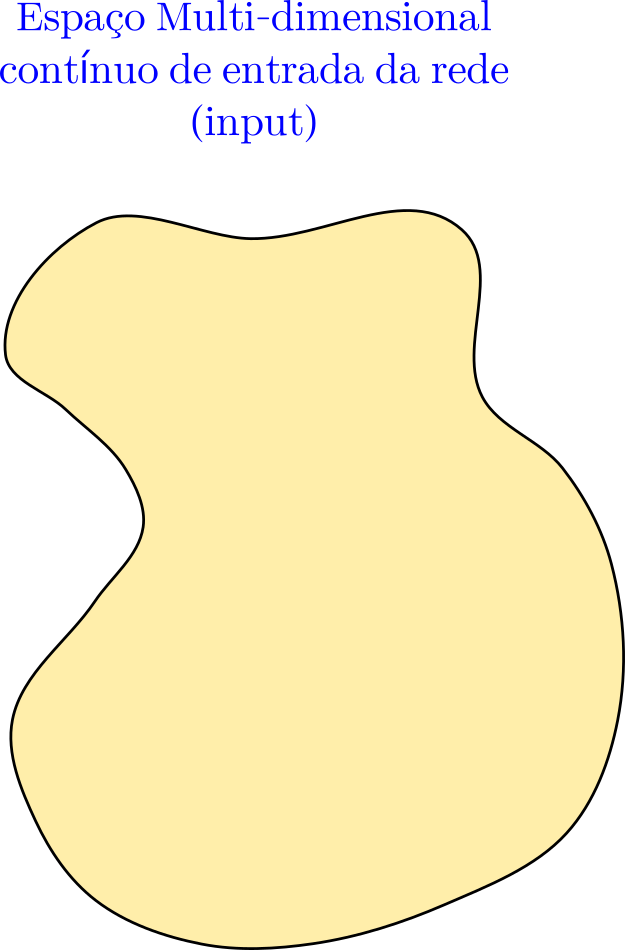
\includegraphics[scale=0.5]{Imagens/IntroKoho1.png} 
	
\end{frame}


\begin{frame}
	\frametitle{A rede de Kohonen}
	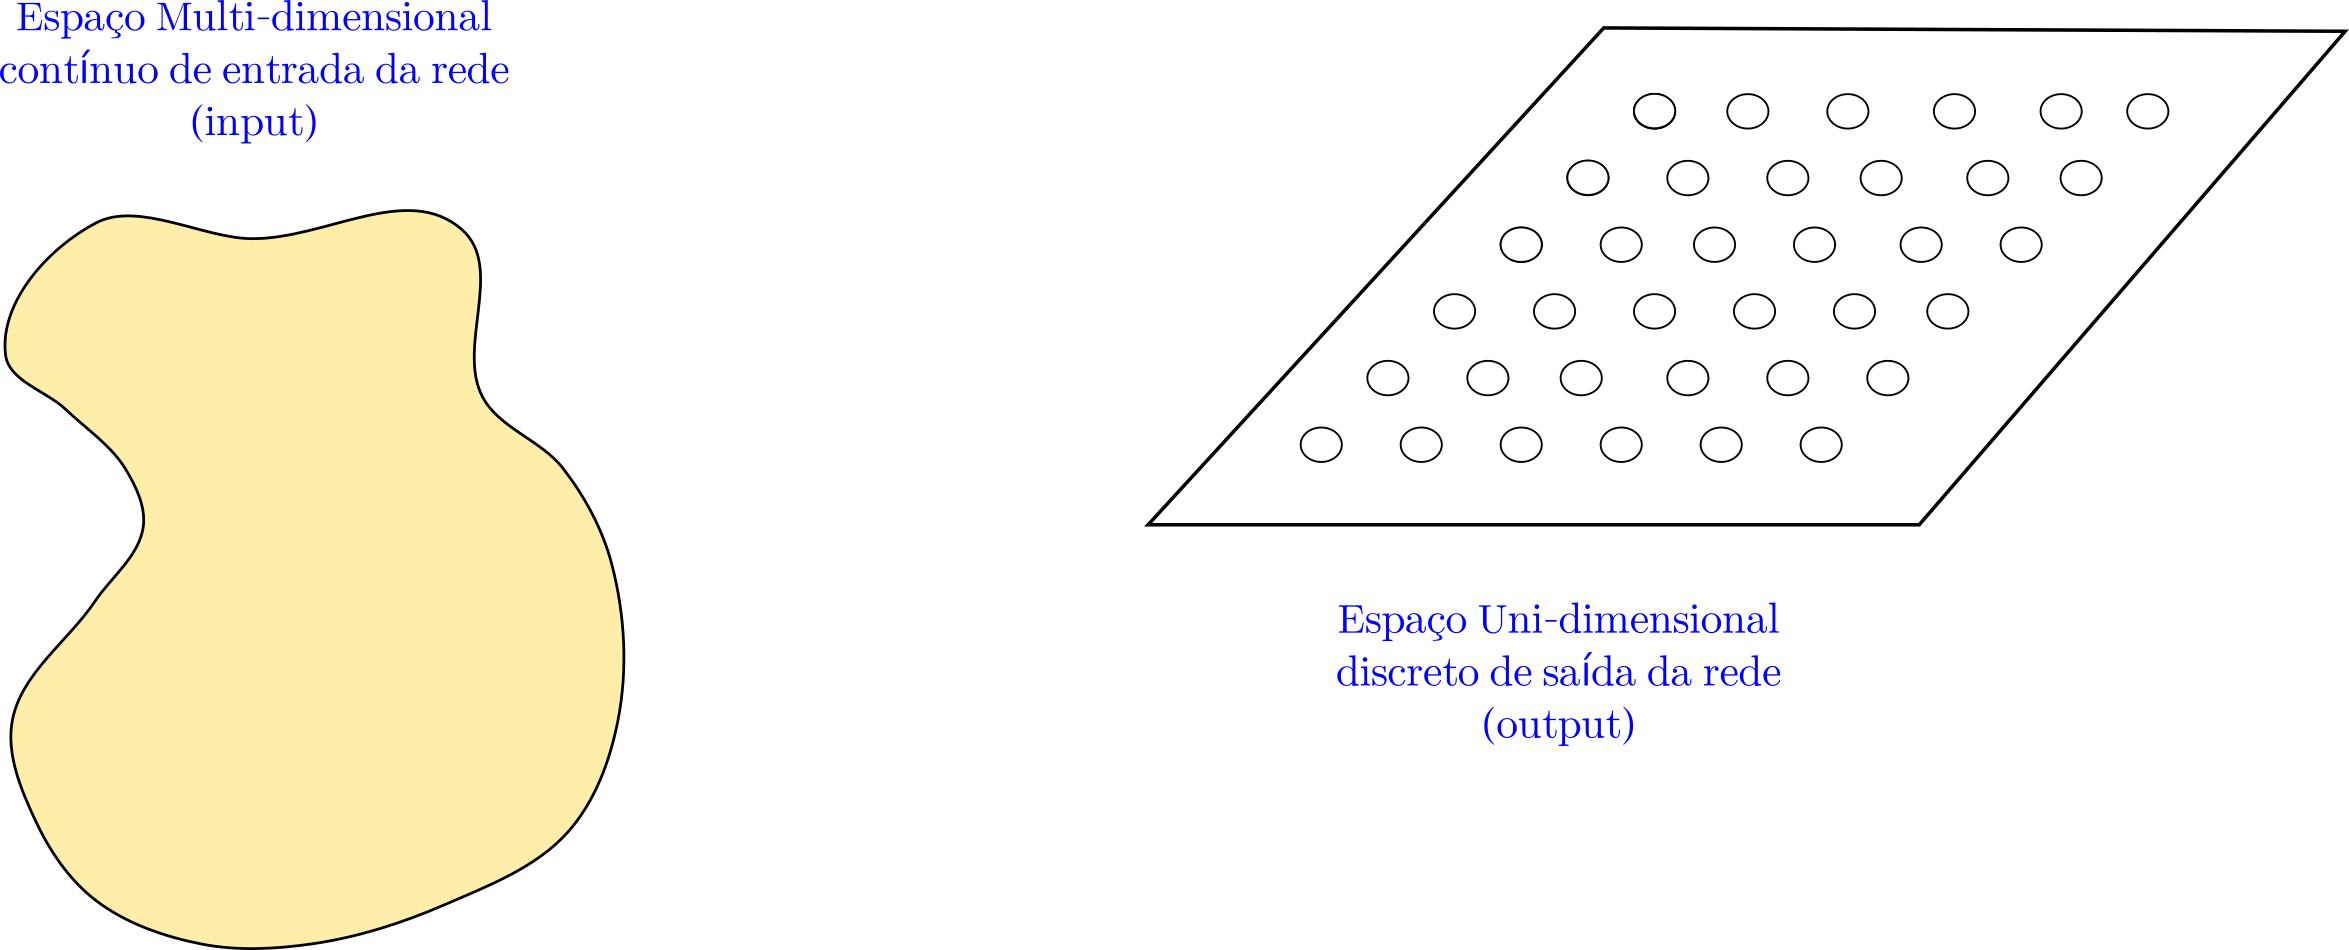
\includegraphics[scale=0.5]{Imagens/IntroKoho2.png} 
	
\end{frame}


\begin{frame}
	\frametitle{A rede de Kohonen}
	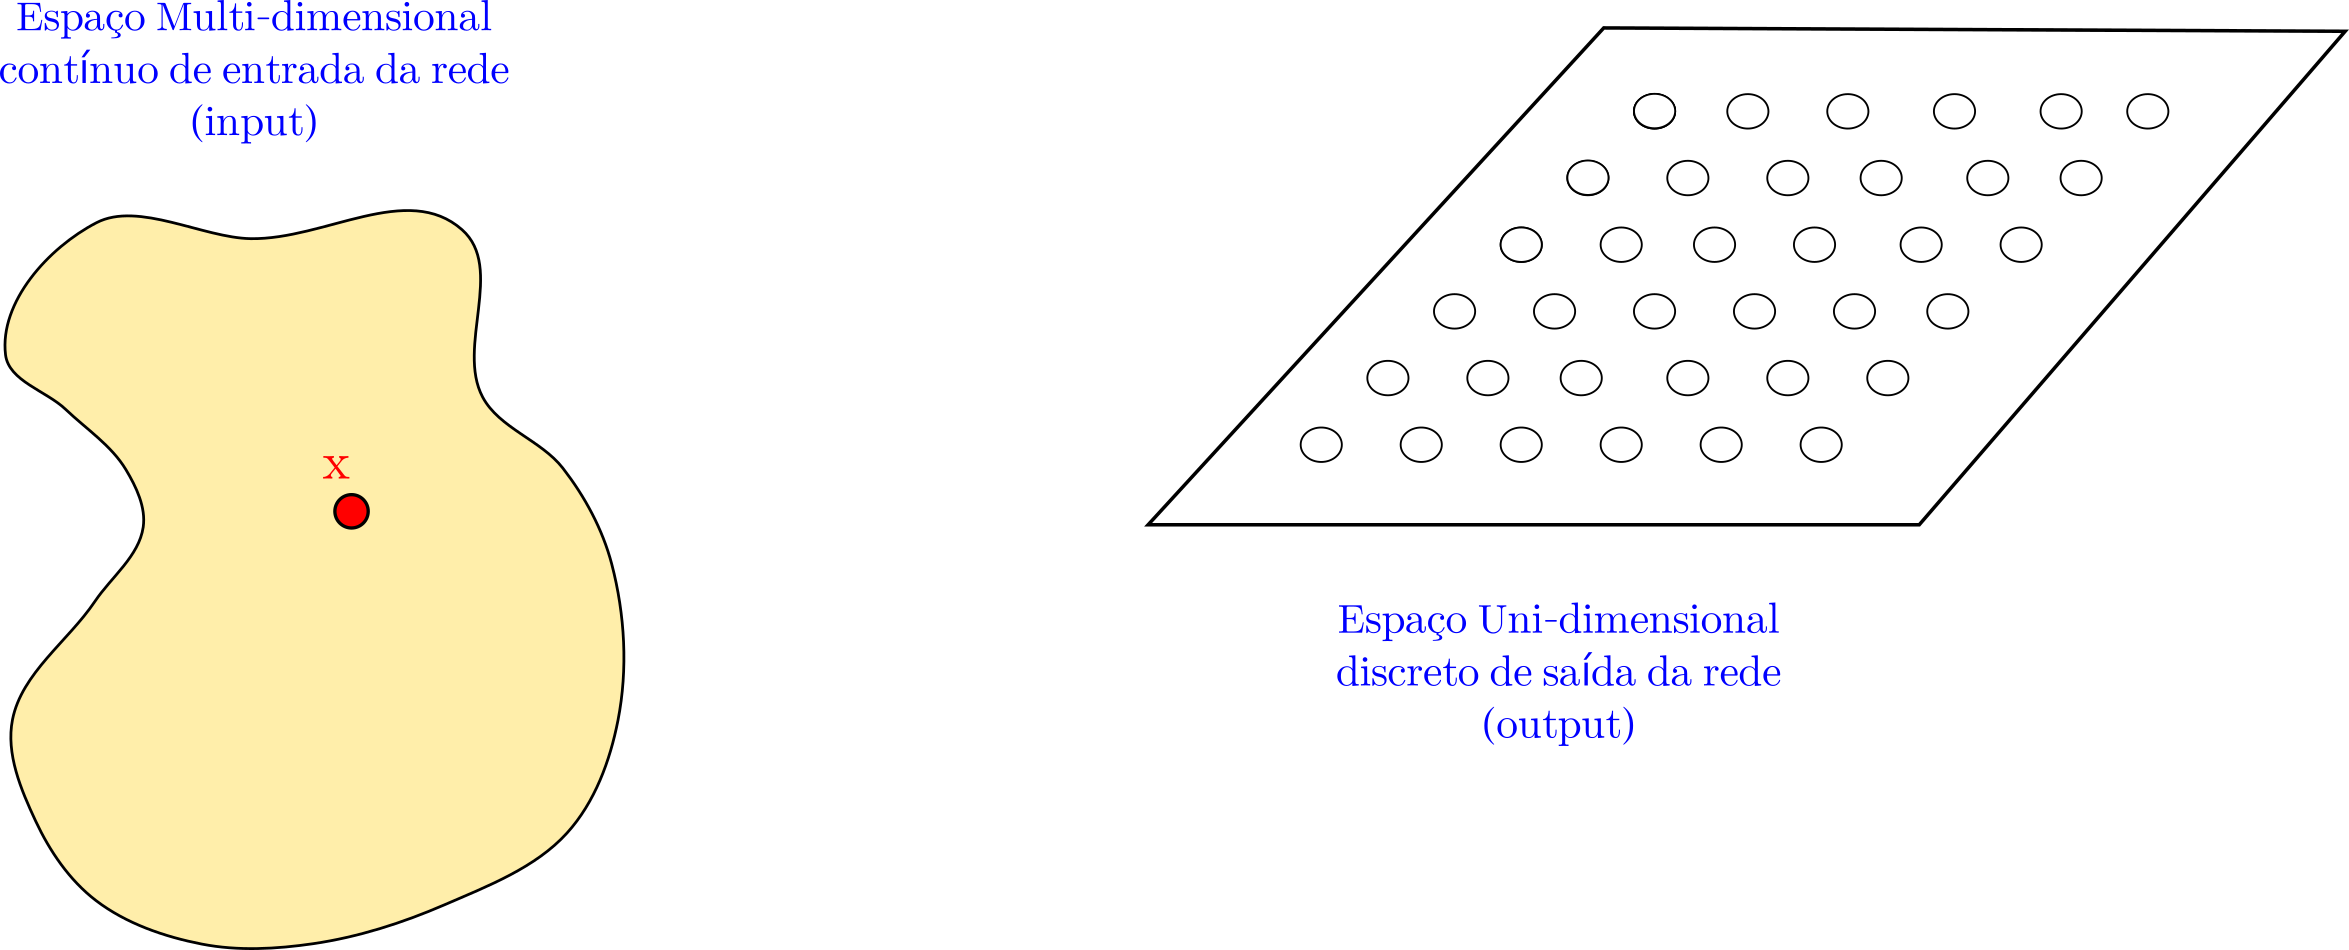
\includegraphics[scale=0.5]{Imagens/IntroKoho3.png} 
	
\end{frame}

\begin{frame}
	\frametitle{A rede de Kohonen}
	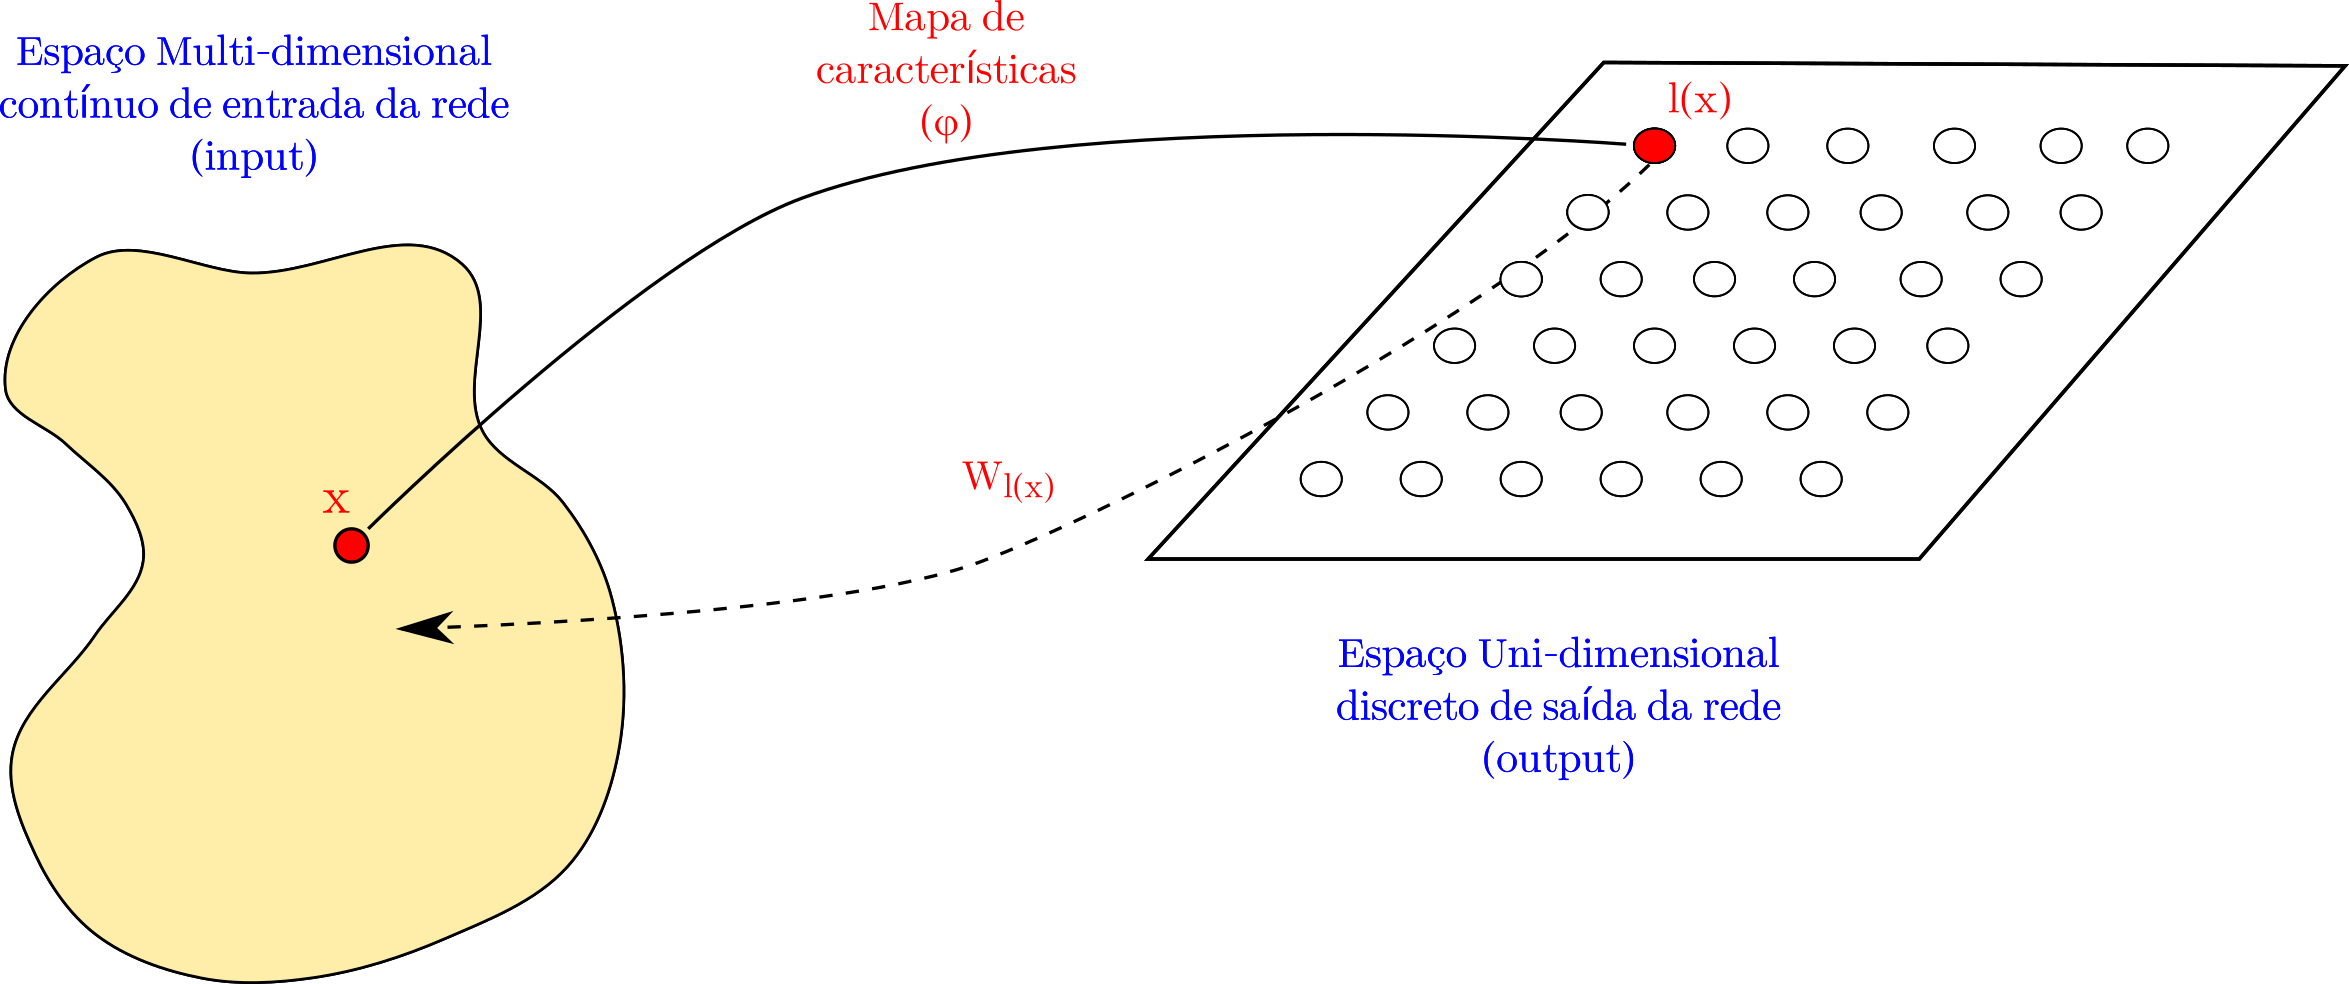
\includegraphics[scale=0.5]{Imagens/IntroKoho4.png} 
	
\end{frame}


\subsection{Treinamento não-supervisionado}

\subsection{Arquitetura da rede}


%%%%%%%%%%%%%%%%%%%%%%%%%%%%%%%%%%%%%%%%%%%%%%%%%%%%%%%%%%%%%%%%%%%%%%%%%%%%
%---------------------------------MODELO------------------------------------
%%%%%%%%%%%%%%%%%%%%%%%%%%%%%%%%%%%%%%%%%%%%%%%%%%%%%%%%%%%%%%%%%%%%%%%%%%%%

\section{Modelo}

\subsection{Fluxogramas}

\subsection{Clusterização}

\subsection{Apresentação dos dados sintéticos}

%%%%%%%%%%%%%%%%%%%%%%%%%%%%%%%%%%%%%%%%%%%%%%%%%%%%%%%%%%%%%%%%%%%%%%%%%%%%
%--------------------------TREINAMENTO DA REDE------------------------------
%%%%%%%%%%%%%%%%%%%%%%%%%%%%%%%%%%%%%%%%%%%%%%%%%%%%%%%%%%%%%%%%%%%%%%%%%%%%

\section{Treinamento da rede}

%%%%%%%%%%%%%%%%%%%%%%%%%%%%%%%%%%%%%%%%%%%%%%%%%%%%%%%%%%%%%%%%%%%%%%%%%%%%
%---------------------------FUNCIONALIDADE DA REDE--------------------------
%%%%%%%%%%%%%%%%%%%%%%%%%%%%%%%%%%%%%%%%%%%%%%%%%%%%%%%%%%%%%%%%%%%%%%%%%%%%

\section{Funcionalidade da rede}

\subsection{Erro}

\subsection{Gráfico de convergência}

%%%%%%%%%%%%%%%%%%%%%%%%%%%%%%%%%%%%%%%%%%%%%%%%%%%%%%%%%%%%%%%%%%%%%%%%%%%%
%-------------------------CRONOGRAMA---------------------------------------
%%%%%%%%%%%%%%%%%%%%%%%%%%%%%%%%%%%%%%%%%%%%%%%%%%%%%%%%%%%%%%%%%%%%%%%%%%%%

\section{Cronograma}		
\begin{frame}
\frametitle{Cronograma}
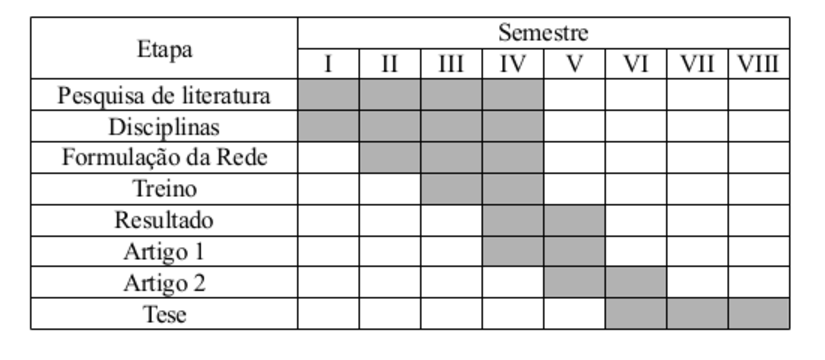
\includegraphics[scale=0.7]{Imagens/Cronograma.pdf} 

\end{frame}

	
\section{Bibliografia}
	\begin{frame}[allowframebreaks]{Bibliografia}
	%\frametitle{Bibliografia}
	\beamertemplatetextbibitems
	\tiny
	\bibliographystyle{apalike}
	\bibliography{referencias.bib}
	\end{frame}

\makeatother
{\nologo
\begin{frame}
%\titlepage
\begin{figure}

\includegraphics[scale=0.25]{Imagens/logonvertical.jpg}
\end{figure}
\begin{center}
\begin{minipage}{0.77\textwidth}
\small
\begin{center}
Rua General José Cristino, 77 CEP 20921-400\\
Rua General Bruce, 586 CEP 20921-030\\
Bairro Imperial de São Cristóvão, Rio de Janeiro - RJ\\
PABX: 55 21 3504-9100\\
\url{www.on.br}
\end{center}
\end{minipage}
\end{center}
\end{frame}
}
\end{document}
